To prepare the camera data for data analysis, the next step in the post-processing workflow involves ``unwrapping'' the cone image; transforming the
hyperbolic shape on the image sensor into a straight one.  The unwrapping step
is accomplished using the software program Fiji~\cite{schindelin2012fiji} and a
straightening algorithm based on cubic spline
interpolation~\cite{kocsis1991image}.  The procedure is depicted in \Figure{fig:extractspklineschematic}.  
\begin{figure}[ht]
\centering
\import{includes/}{setpgfinc}
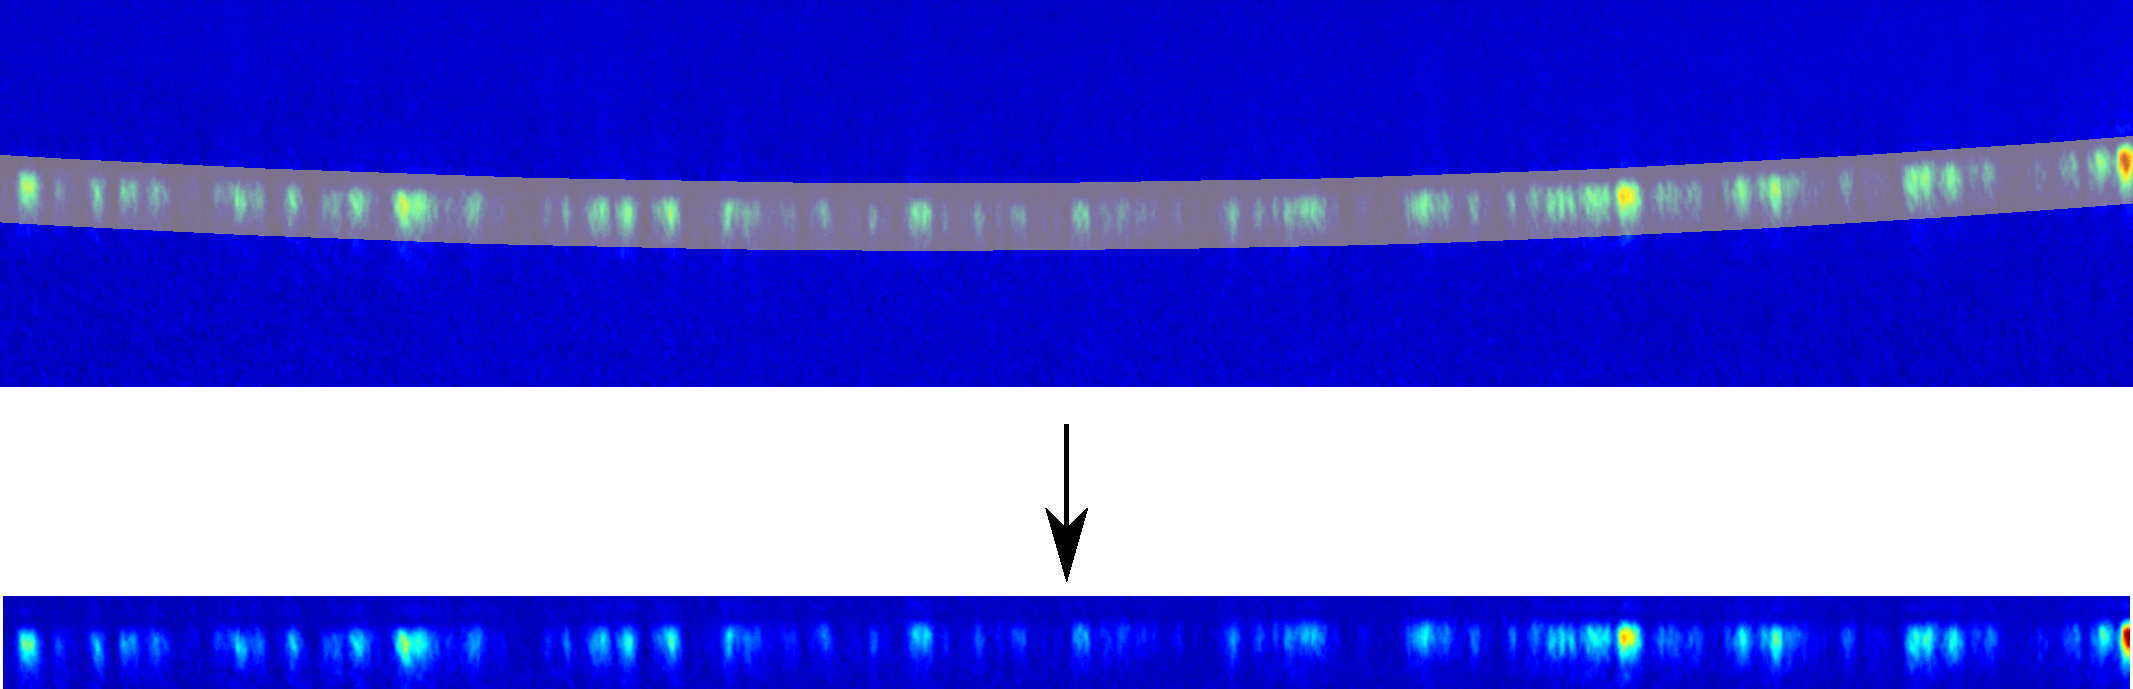
\includegraphics[keepaspectratio,width=15cm]{experimental/figures/extractspkline.pdf}
\caption{Illustration of the unwrapping procedure for the cone image.  The spline region (highlighted in yellow) in the above image is converted to the rectangular region in the image below for further post-processing.}
\label{fig:extractspklineschematic}
\end{figure}
